\section{Motivation}
With the advances in technology, the human race was able to establish dominance over the creatures of the planet. Now issues of survival due to micro (ref bacteria viruses, disease), and macro - the chaning climate and food supply.

As part of this air pollution and climate have always been a concern for the human race. Concerns about lead in the air can be documented back as far as 6000 years ago [se ref, ], in ancient Rome [1145] and in 1285 where after a visit from Queen of England to a coal burning to Nottingham, the first air pollution act was deployed [1147].

air pollution = animals

air qulaity pollicy
kingxx




\section{composition of the atmosphere}

Paper atmospere

main o2 and N ,
however billions
each of these can be responsible for other reactions.

Mention OH mention O3 and pans
Mention lifetimes.




\section{Changing Climate}



The main removal

\subsection{HOx Cycle}





\section{Air Quality}


\begin{figure}[H]
  \centering
  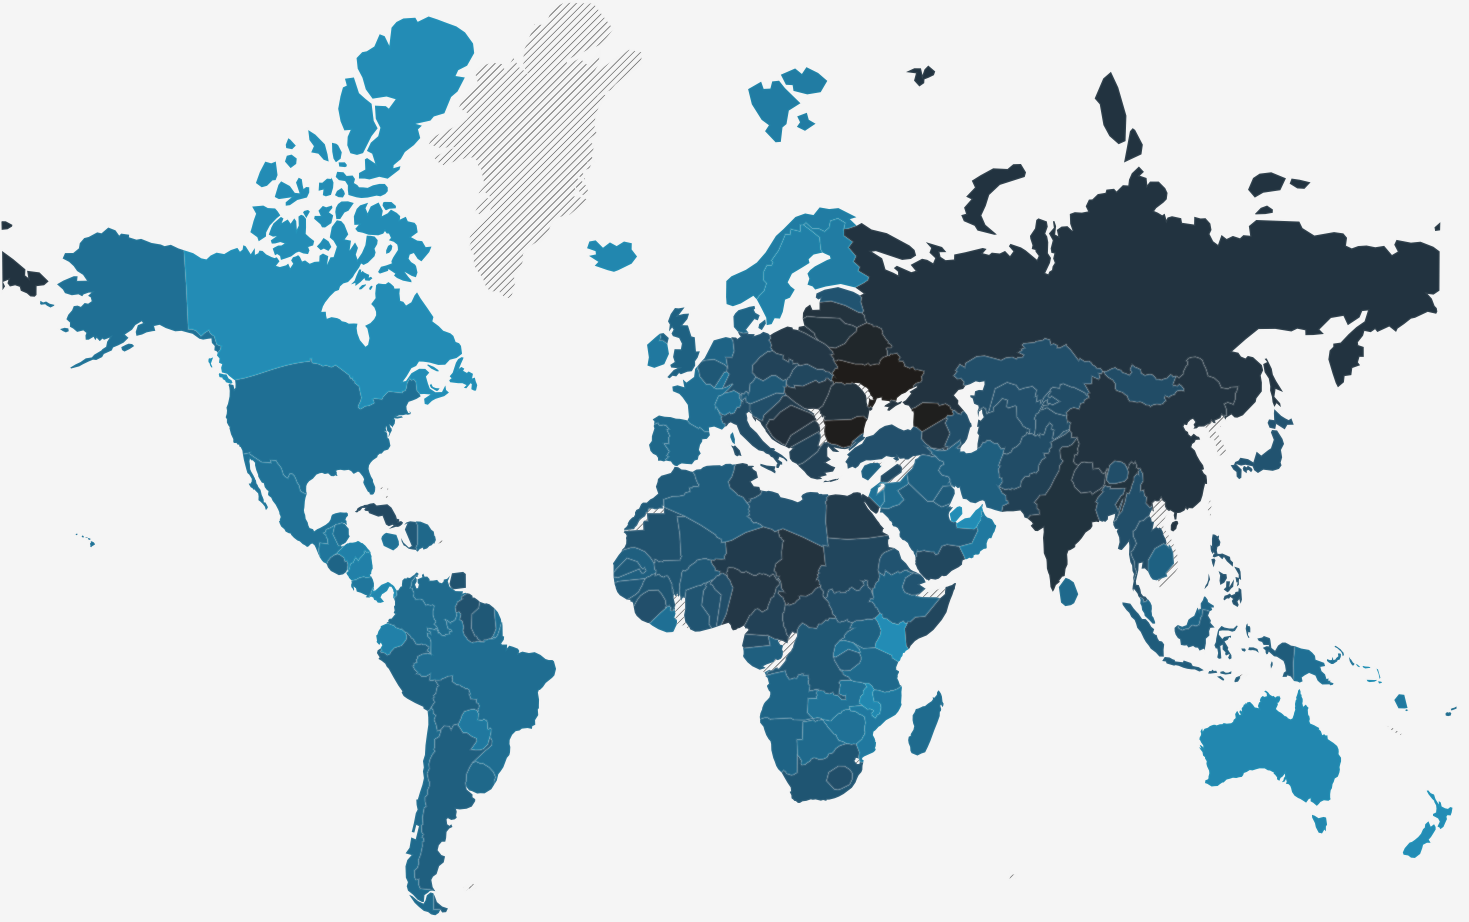
\includegraphics[width=\textwidth]{who.png}
  \caption{\textbf{Deaths attributed to air pollution REF WHO 16}}
  \label{fig:who}
\end{figure}

\section{Ozone and its role}
Ozone has two roles within the atmosphere. High up in the stratosphere it servers as a barrier to dangerous ultraviolet radiation. The importance of this was discovered in (HOLE PAPER) where the release of CloroFlouroCarbons from deodorants produced ...

However within the troposhere (<15k?) the production and loss of ozone has a direct impact on human life. Polluted environments, such as industrial London,
SMOG, Clean air act.



\section{The NOx cycle}
Nitrogen Oxides (NOx) come predominantly from motor verhicles and power stations and can cause respiotory problems in children and asmatics [se1261]. They also play an important role in the formation and destruction of ozone.








VOC
